\documentclass[aspectratio=169]{beamer}
\usepackage{tikz}
\usepackage{siunitx}

\title{Extension of the Adaptable Seismic Data Format (ASDF) for Applications in Engineering Seismology}
\subtitle{}
\author{Brad Aagaard$^1$, Mike Hearne$^2$, Albert Kottke$^3$, Eric Thompson$^2$, Jamie Steidl$^1$}
\institute{
\includegraphics[height=10mm]{../logos/USGSL}\hspace*{2cm}
\includegraphics[height=12mm]{../logos/pge}}
\date{April 25, 2019\\[6mm]
  \begin{minipage}{\textwidth}
  {\footnotesize
  $^1$ U.S. Geological Survey, Menlo Park, CA\\
  $^2$ U.S. Geological Survey, Golden, CO\\
    $^3$Pacific Gas \& Electric}
  \end{minipage}}

% ---------------------------------------------------- CUSTOMIZATION
\usetheme{USGS}
\usecolortheme{usgsdark}
\setbeamercolor{note text}{fg=ltpurple}

\newcommand{\includefigure}[2][]{{\centering\includegraphics[#1]{#2}\par}}

\newcommand{\highlight}[1]{{\bf\usebeamercolor[fg]{note text}#1}}
\newcommand{\remark}[1]{{\usebeamercolor[fg]{highlight}#1}}
\newcommand{\credit}[1]{{\itshape\footnotesize#1}}
\newcommand{\todo}[1]{{\color{ltred}\bfseries TODO: #1}}

\usetikzlibrary{arrows,shapes,calc}
\newcommand{\tikzmark}[1]{\tikz[remember picture,overlay,baseline=-0.5ex] \coordinate (#1);}
\tikzstyle{popup-figure} = [thick,
  rectangle callout, callout absolute pointer={#1}, anchor=center,
  font=\mdseries, draw=usgs_yellow,
  fill=black, fill opacity=0.85, text opacity=1.0, text=white]

% From http://communities.usgs.gov/blogs/vis/typography-and-color/additional-colors/

% Main Colors
\definecolor{usgs_green}{HTML}{006F41}
\definecolor{usgs_teal}{HTML}{0061A3}
\definecolor{usgs_blue}{HTML}{0071B7}
\definecolor{usgs_navy}{HTML}{180F9B}
\definecolor{usgs_purple}{HTML}{8F009A}
\definecolor{usgs_red}{HTML}{FB0032}
\definecolor{usgs_orange}{HTML}{F99B00}

% USGS Dark Colors
\definecolor{usgs_dkgreen}{HTML}{1E4D2B}
\definecolor{usgs_dkgreen2}{HTML}{00443F}
\definecolor{usgs_dkblue}{HTML}{002F57}
\definecolor{usgs_dknavy}{HTML}{201258}
\definecolor{usgs_dkpurple}{HTML}{641B56}
\definecolor{usgs_dkred}{HTML}{881535}
\definecolor{usgs_dkorange}{HTML}{8D4200}


% USGS Light and Neutral Colors
\definecolor{usgs_ltblue}{HTML}{6AC3F2}
\definecolor{usgs_yellow}{HTML}{FFBD00}
\definecolor{usgs_ltgreen}{HTML}{66A48B}
\definecolor{usgs_ltgray}{HTML}{91B0BD}


\definecolor{ltyellow}{rgb}{1.0, 1.0, 0.45} % 255/255/115
\definecolor{yellow}{rgb}{0.9, 0.9, 0.0} % % 230/230/0

\definecolor{ltorange}{rgb}{1.0, 0.74, 0.41} % 255/188/105
\definecolor{orange}{rgb}{0.96, 0.50, 0.0} % 246/127/0

\definecolor{ltred}{rgb}{1.0, 0.25, 0.25} % 255/64/64
\definecolor{red}{rgb}{0.79, 0.00, 0.01} % 201/0/3

\definecolor{ltpurple}{rgb}{0.81, 0.57, 1.00} % 206/145/255
\definecolor{purple}{rgb}{0.38, 0.00, 0.68} % 97/1/175

\definecolor{ltblue}{rgb}{0.67, 0.85, 0.91} % 171/217/233
\definecolor{blue}{rgb}{0.17, 0.48, 0.71} % 44/123/182

\definecolor{ltltgreen}{rgb}{0.7, 1.00, 0.7} % 96/204/14
\definecolor{ltgreen}{rgb}{0.37, 0.80, 0.05} % 96/204/14
\definecolor{green}{rgb}{0.23, 0.49, 0.03} % 59/125/8
  
\definecolor{dkslate}{rgb}{0.18, 0.21, 0.28} % 47/53/72
\definecolor{mdslate}{rgb}{0.45, 0.50, 0.68} % 114/127/173
\definecolor{ltslate}{rgb}{0.85, 0.88, 0.95} % 216/225/229

\definecolor{dkgray}{rgb}{0.25, 0.25, 0.25}
\definecolor{mdgray}{rgb}{0.50, 0.50, 0.50}
\definecolor{ltgray}{rgb}{0.75, 0.75, 0.75}




% --------------------------------------------------------- DOCUMENT
\begin{document}

% ------------------------------------------------------------ SLIDE
\maketitle

\logo{
\includegraphics[height=7.0ex]{../logos/pge}
\includegraphics[height=4.5ex]{../logos/USGSLsimple}}

% ========================================================== SECTION
\section{Introduction}

% ------------------------------------------------------------ SLIDE
\begin{frame}
  \frametitle{Summary}
  \summary{}

  \highlight{We propose an extension to the Adaptable Seismic Data
    Format (ASDF) for storing ground-motion intensity metrics for
    engineering seismology applications.}

  \begin{itemize}
  \item \remark{Single file}
    \begin{itemize}
    \item Earthquake source
    \item Ground-motion waveforms and station metadata
    \item Intensity and station metrics
    \item Provenance information
    \end{itemize}
  \item \remark{Build upon Adaptable Seismic Data Format (ASDF)}
    \begin{itemize}
    \item Leverages commonly used portable, binary files (HDF5) with high-level interfaces
    \item Leverages standards from seismological community (QuakeML, StationXML)
    \item Adds waveform and station metrics to AuxiliaryData
    \end{itemize}
  \end{itemize}
  
\end{frame}


% ------------------------------------------------------------ SLIDE
\begin{frame}
  \frametitle{Motivation}
  \summary{Improve data management for engineering seismology applications}

  \begin{itemize}
  \item \remark{Collect data into a single container}
    \begin{itemize}
    \item Data comes from multiple sources in different formats
    \item Need a record of data source and processing (provenance information)
    \end{itemize}
  \item \remark{Storage of both raw and processed data}
    \begin{itemize}
    \item Want to compute additional intensity metrics, starting from processed waveforms
    \item Reprocess data with new or alternative algorithms
    \end{itemize}
  \end{itemize}

\vfill
See {\bf Poster 109}: Community-Supported Ground-Motion Processing Software
    
\end{frame}


% ------------------------------------------------------------ SLIDE
\begin{frame}
  \frametitle{Workflow}
  \summary{Workspace holds data for ground-motion processing workflow}

  \includefigure[width=\textwidth]{figs/workspace}

\end{frame}


% ------------------------------------------------------------ SLIDE
\begin{frame}
  \frametitle{Storage Layout: Why HDF5?}
  \summary{HDF5 is a widely used scientific data format}

  \begin{itemize}
  \item \remark{HDF5 originally developed for supercomputing}
  \item \remark{Supports wide variety of data and attributes}
    \begin{itemize}
    \item Store data and metadata in a single file
    \end{itemize}
  \item \remark{Standard binary format with high-level interfaces (Python, R, Matlab, etc.)}
    \begin{itemize}
      \item Example: Get dataset (array) via Python:\\
        \includefigure[scale=0.4]{figs/why_hdf5}
    \end{itemize}
  \item \remark{Extensible}
    \begin{itemize}
    \item Add groups and datasets without affecting existing tree structure
    \end{itemize}
  \end{itemize}
  
\end{frame}


% ========================================================== SECTION
\section{ASDF}

% ------------------------------------------------------------ SLIDE
\begin{frame}
  \frametitle{Adaptable Seismic Data Format (ASDF), Krischer et al. 2016}
  \summary{Store seismic waveform data plus source and station metadata in a single file}

  \highlight{From Krischer et al. (2016):}

  \begin{itemize}
  \item \remark{Provides a well-defined format for storing and exchanging seismological data sets, including all necessary meta information}
    \begin{itemize}
    \item Track and store history of data (provenance)
    \end{itemize}
  \item \remark{Works equally well for recorded and synthetic data}
  \item \remark{Single file improves computational performance and workflow}
    \begin{itemize}
    \item Efficient parallel input/output
    \item Transparent lossless compression
    \item Extensible, portable, self-describing format
    \end{itemize}
  \end{itemize}
 
\end{frame}


% ------------------------------------------------------------ SLIDE
\begin{frame}
  \frametitle{Use Cases for Extended ASDF}
  \summary{}

  \begin{itemize}
  \item \remark{Add engineering metrics (PGA, PSA, EAS, etc.) to the ASDF container}
    \begin{itemize}
    \item Common structure to aid collaboration and reduce rework
    \item Store provenance information for quality assurance
    \end{itemize}
  \item \remark{Analysis of recorded or synthetic ground-motion waveforms}
    \begin{itemize}
    \item Facilitates reprocessing of old records with new algorithms without overwriting
    \end{itemize}
  \item \remark{USGS ShakeMap production}
    \begin{itemize}
    \item Incorporate data from multiple sources (raw waveforms, processed waveforms, intensity)
    \item Easy to add additional metrics and rebuild ShakeMap input
    \end{itemize}
  \item \remark{Archiving}
    \begin{itemize}
    \item Original waveforms through intensity measures with provenance
    \item Synthetic waveforms with rupture models and provenance
    \end{itemize}
  \end{itemize}
  
\end{frame}


% ------------------------------------------------------------ SLIDE
\begin{frame}[t]
  \frametitle{ASDF Layout}
  \summary{Hierarchical organization of waveforms and earthquake and station metadata}

  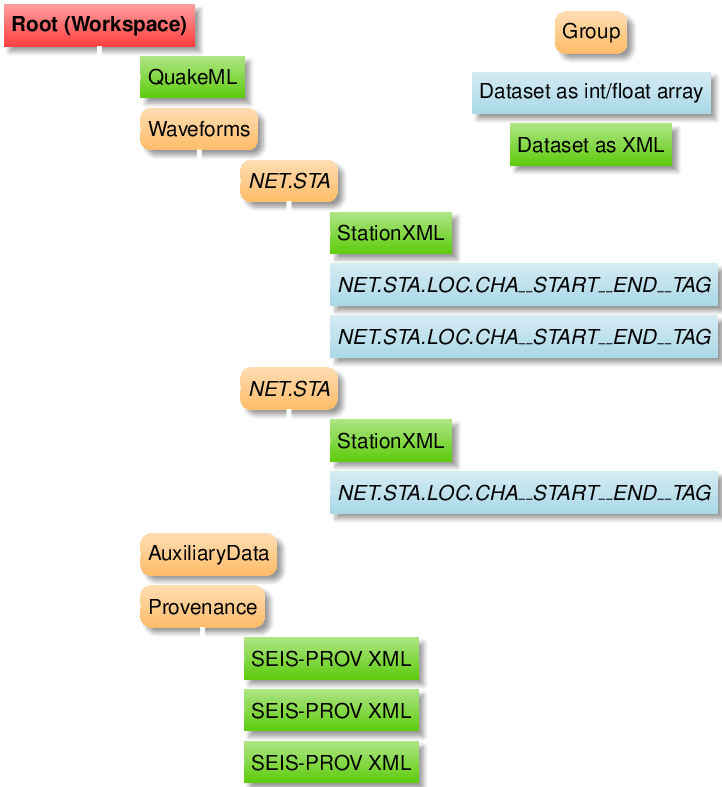
\includegraphics[scale=0.5]{figs/asdf_layout_summary}
  
\end{frame}


% ------------------------------------------------------------ SLIDE
\begin{frame}[t]
  \frametitle{ASDF: Earthquake Source}
  \summary{Earthquake source information stored as QuakeML}

  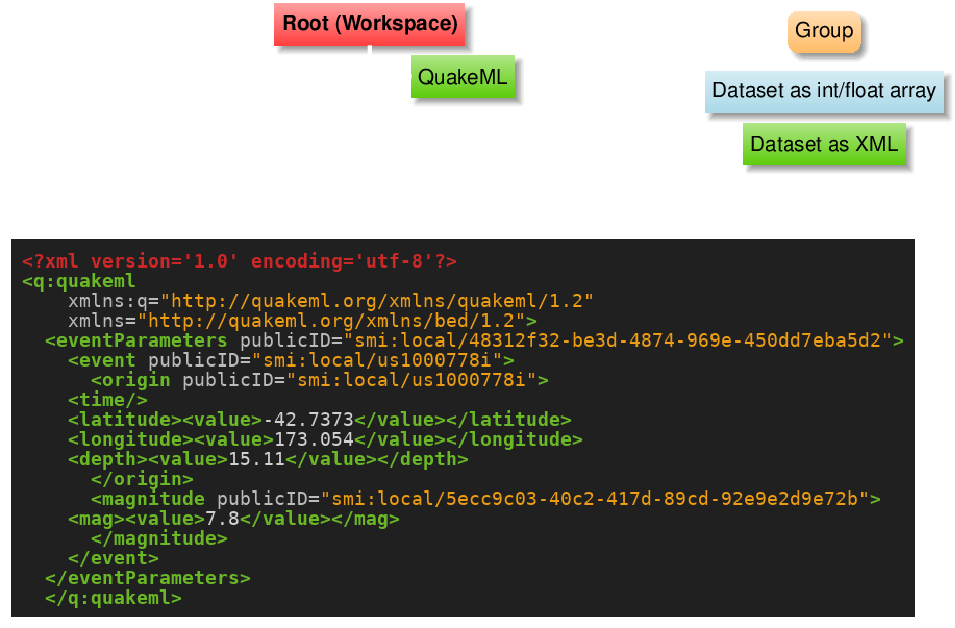
\includegraphics[scale=0.5]{figs/asdf_layout_eqsrc}

  \begin{tikzpicture}[remember picture, overlay]
    \node<2>[popup-figure={(2,1)}] at (0.5\textwidth,-2.0) {
      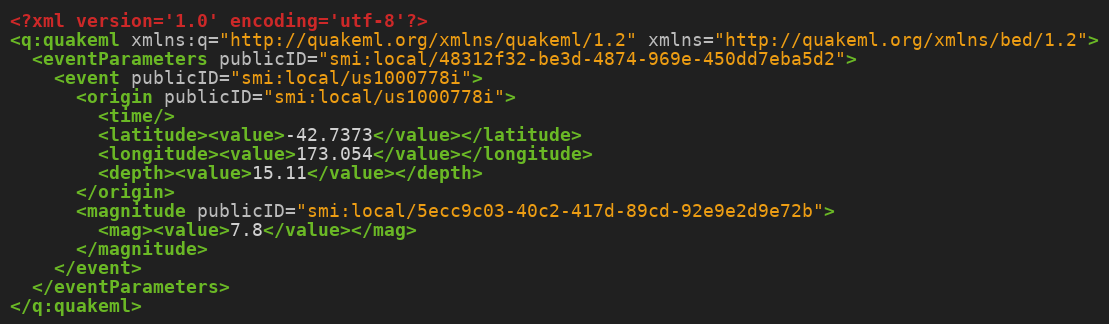
\includegraphics[scale=0.30]{figs/asdf_quakeml}};
  \end{tikzpicture}
  
\end{frame}


% ------------------------------------------------------------ SLIDE
\begin{frame}[t]
  \frametitle{ASDF: Waveforms}
  \summary{Metadata as StationXML; waveforms as float arrays}

  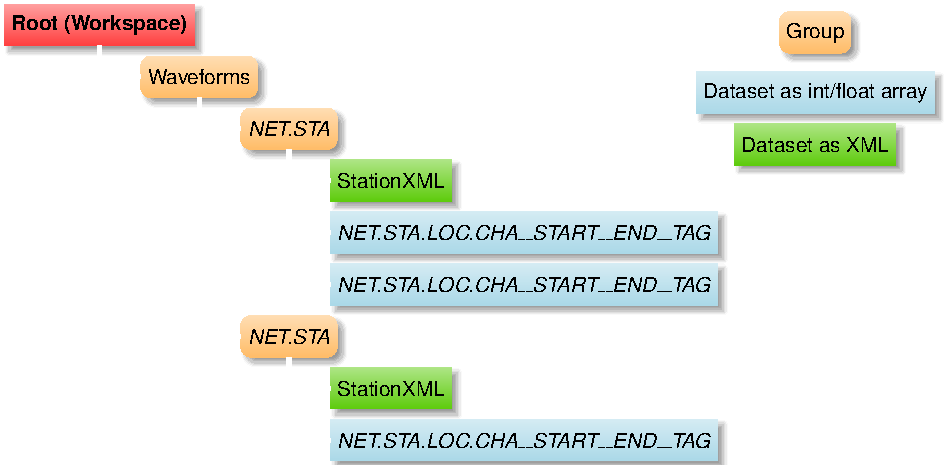
\includegraphics[scale=0.5]{figs/asdf_layout_waveforms}
  
\end{frame}


% ------------------------------------------------------------ SLIDE
\begin{frame}[t]
  \frametitle{ASDF: Provenance Information}
  \summary{Provenance information stored as SEIS-PROV (extension of W3C PROV)}

  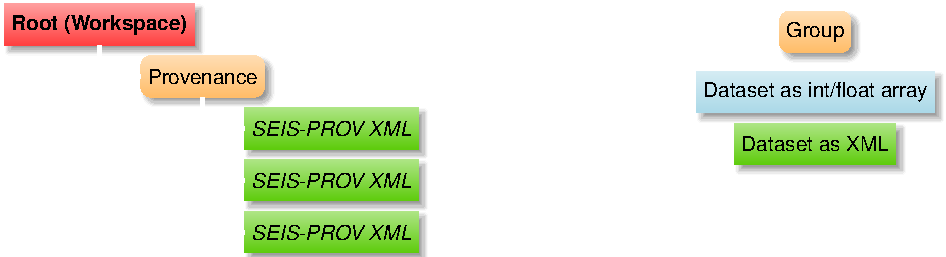
\includegraphics[scale=0.5]{figs/asdf_layout_provenance}
  
  \begin{tikzpicture}[remember picture, overlay]
    \node<2>[popup-figure={(2,2)}] at (0.5\textwidth,-1.0) {
      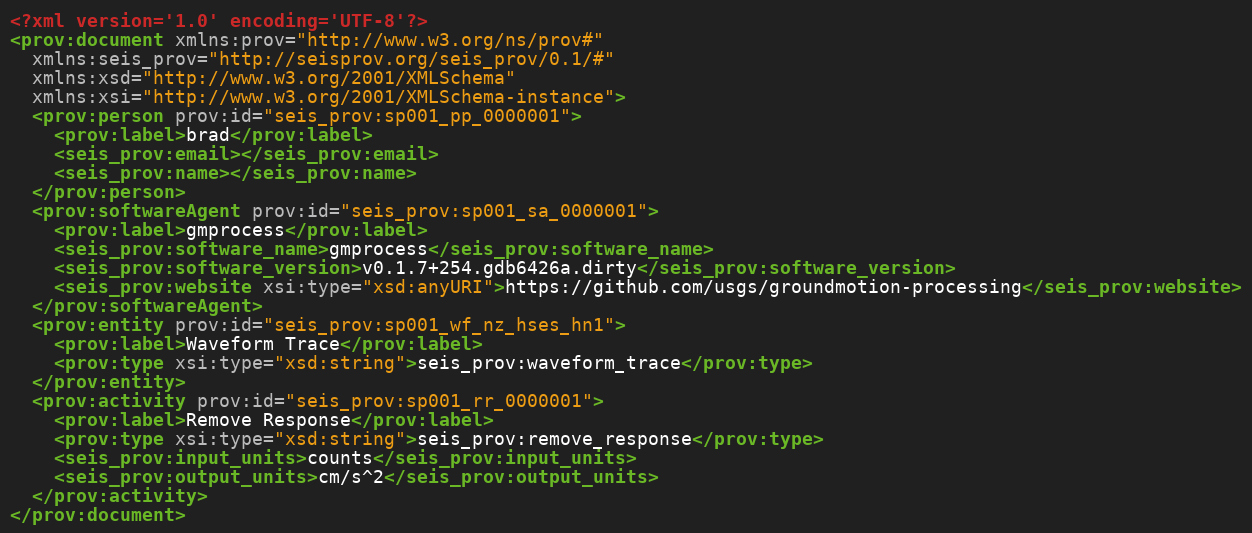
\includegraphics[scale=0.30]{figs/asdf_provxml}};
  \end{tikzpicture}
  
\end{frame}


% ========================================================== SECTION
\section{Extended ASDF}

% ------------------------------------------------------------ SLIDE
\begin{frame}[t]
  \frametitle{Extending ASDF: Waveform Metrics}
  \summary{One waveform metrics dataset per station and processing tag}

  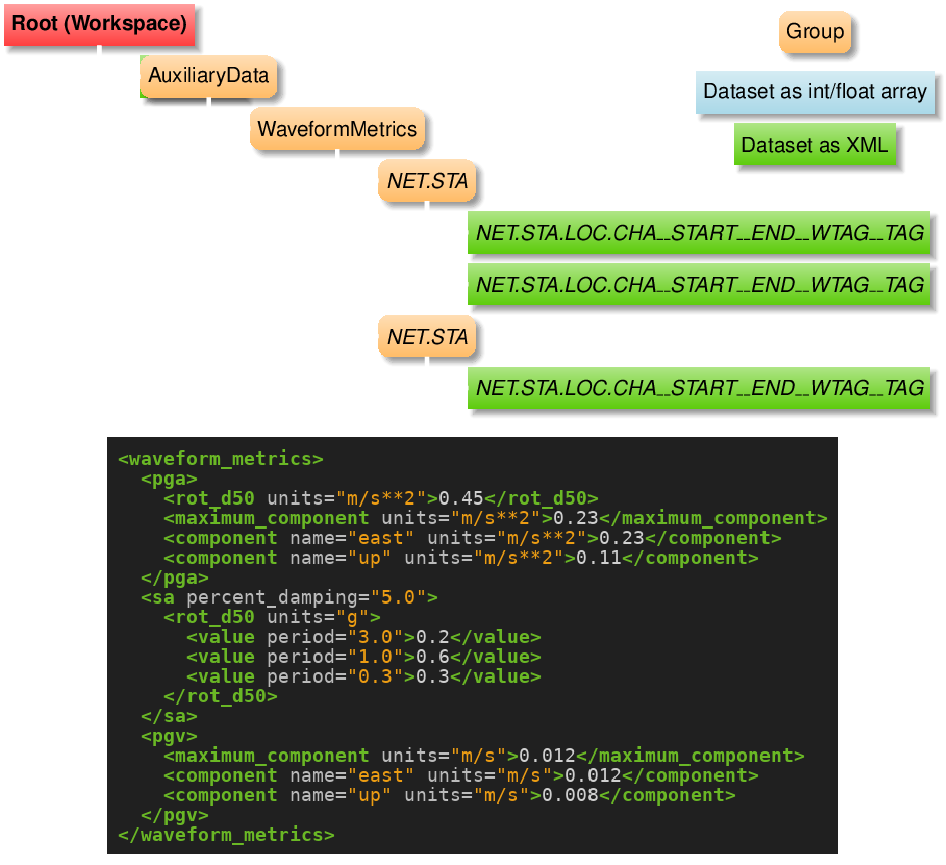
\includegraphics[scale=0.5]{figs/asdf_layout_waveformmetrics}
  
  \begin{tikzpicture}[remember picture, overlay]
    \node<2>[popup-figure={(5,2)}] at (0.7\textwidth,0.0) {
      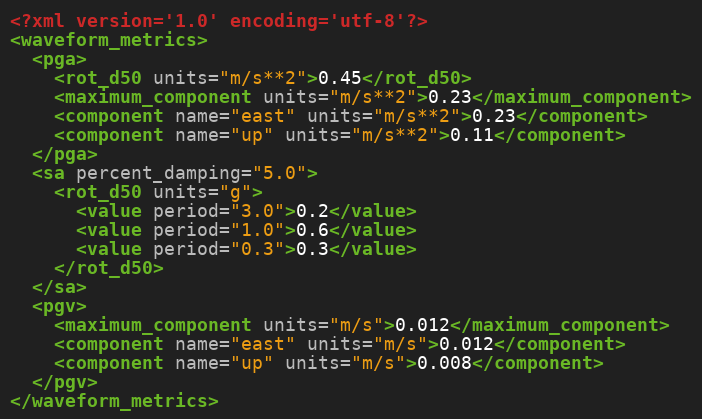
\includegraphics[scale=0.30]{figs/asdf_waveformmetricsxml}};
  \end{tikzpicture}
  
\end{frame}


% ------------------------------------------------------------ SLIDE
\begin{frame}[t]
  \frametitle{Extending ASDF: Station Metrics}
  \summary{One station metrics dataset per event and rupture model}

  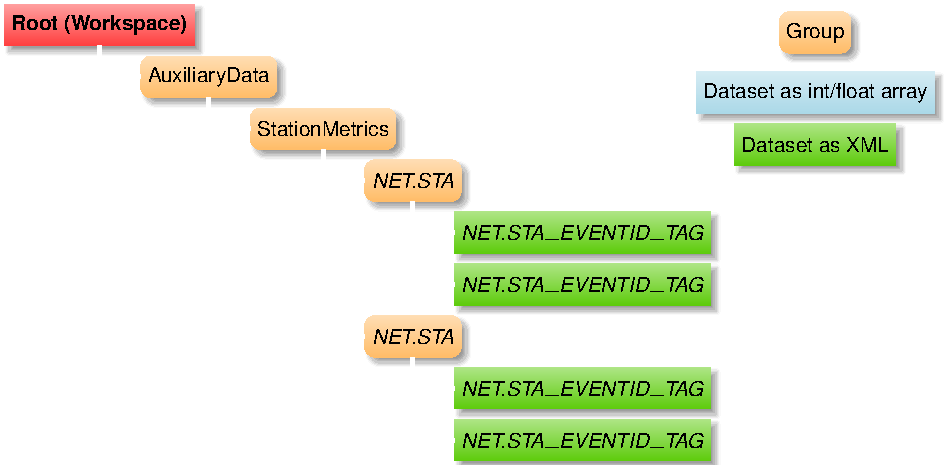
\includegraphics[scale=0.5]{figs/asdf_layout_stationmetrics}
  
  \begin{tikzpicture}[remember picture, overlay]
    \node<2>[popup-figure={(5,2)}] at (0.7\textwidth,0.0) {
      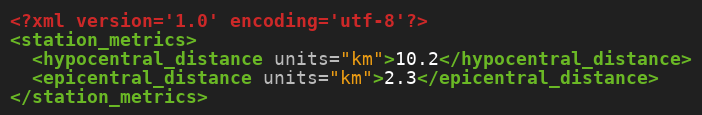
\includegraphics[scale=0.30]{figs/asdf_stationmetricsxml}};
  \end{tikzpicture}
  
\end{frame}


% ------------------------------------------------------------ SLIDE
\begin{frame}
  \frametitle{Example: Import Waveforms and Metadata}
  \summary{Using USGS {\tt groundmotion-processing} software (see Poster 109)}

  \includefigure[scale=0.45]{figs/asdf_demo_import}
  
\end{frame}


% ------------------------------------------------------------ SLIDE
\begin{frame}
  \frametitle{Example: Process Waveforms}
  \summary{Using USGS {\tt groundmotion-processing} software (see Poster 109)}

  \includefigure[scale=0.45]{figs/asdf_demo_process}
  
\end{frame}


% ------------------------------------------------------------ SLIDE
\begin{frame}
  \frametitle{Example: Retrieving Data from Workspace}
  \summary{Using USGS {\tt groundmotion-processing} software (see Poster 109)}

  \includefigure[scale=0.45]{figs/asdf_demo_query}
  
\end{frame}


% ========================================================== SECTION
\section{Summary}

% ------------------------------------------------------------ SLIDE
\begin{frame}
  \frametitle{Summary}
  \summary{Also see {\bf Poster 109}: Community-Supported Ground-Motion Processing Software}

  \highlight{We propose an extension to the Adaptable Seismic Data
    Format (ASDF) for storing ground-motion intensity metrics for
    engineering seismology applications.}

  \begin{itemize}
  \item \remark{Single file}
    \begin{itemize}
    \item Earthquake source
    \item Ground-motion waveforms and station metadata
    \item Intensity and station metrics
    \item Provenance information
    \end{itemize}
  \item \remark{Extend ASDF AuxiliaryData to include waveform and station metrics}
  \item \remark{Let us know what you think}
    \begin{itemize}
    \item Code repository: \url{https://github.com/usgs/groundmotion-processing}
    \item Documentation: \url{https://usgs.github.io/groundmotion-processing}
    \end{itemize}
  \end{itemize}
  
\end{frame}


% --------------------------------------------------------- DOCUMENT
\end{document}

% End of file
